\documentclass[a4paper, oneside]{memoir}
\usepackage[danish]{babel} % load typographical rules for the english language
\usepackage{graphics} % for \scalebox
\usepackage{hyperref} % for \href
\usepackage{xcolor} % for text color
\usepackage{enumitem} % for ordered and unordered list
\usepackage{graphicx} % for images
\usepackage{pdfpages} % for including pdfs
\usepackage{footnote} % for footnotes
\usepackage{longtable} % for tabular environment that spans multiple pages and supports footnotes
\usepackage{colortbl} % for cell coloring
\usepackage{multirow} % for \multicolumn

% https://github.com/latex3/babel/issues/51
\makeatletter\AtBeginDocument{\let\@elt\relax}\makeatother

% styling
\setsecnumdepth{subsubsection} % how deep to number sections
\setlength{\parindent}{0em} % horizontal indent for first line of paragraph
\setlength{\parskip}{1em} % vertical space between paragraphs

\newcommand{\textdesc}[1]{\textit{\textbf{#1}}}
\newcommand{\descitem}[1]{\item \textdesc{#1}}

\title{\documenttitle\\\scalebox{0.85}{\documentsubtitle}}
\author{Aslak Johansen \href{mailto:asjo@mmmi.sdu.dk}{asjo@mmmi.sdu.dk}\\Aisha Umair \href{mailto:aiu@mmmi.sdu.dk}{aiu@mmmi.sdu.dk}}

\begin{document}

\maketitle
\setcounter{tocdepth}{2}
\tableofcontentswrapper


\chapter{Kursushåndbog: Kom godt i gang!}

%%%%%%%%%%%%%%%%%%%%%%%%%%%%%%%%%%%%%%%%%%%%%%%%%%%%%%%%%%%%%%%%%%%%%%%%%%%%%%%%
%%%%%%%%%%%%%%%%%%%%%%%%%%%%%%%%%%%%%%%%%%%%%%%%%%%%%%%%%%%%%%%%%%%%%%%%%%% Hvordan er kurset opbygget på itslearning?
\section{Hvordan er kurset opbygget på itslearning?}
\begin{itemize}
\item Under \textbf{Oversigt (Announcements)} ligger alle meddelelser om kurset, så du til enhver tid kan se både gamle og nye meddelelser. Du får oplysninger om kursusplan og kontaktpersoner som en annoncering.
\item Under \textbf{Planer} ligger kursets moduler, som beskriver alt det du løbende skal gøre i kurset.

\item Under \textbf{Ressourcer} finder du alle de materialer som bruges i kursets moduler. Under ressourcers kan du altså genfinde kursusmaterialer.

\item Under \textbf{Status og opfølgning} kan du se dine fremskridt på kurset.
\end{itemize}

%%%%%%%%%%%%%%%%%%%%%%%%%%%%%%%%%%%%%%%%%%%%%%%%%%%%%%%%%%%%%%%%%%%%%%%%%%%%%%%%
%%%%%%%%%%%%%%%%%%%%%%%%%%%%%%%%%%%%%%%%%%%%%%%%%%%%%%%%%%%%%%%%%%%%%%%%%%% Hvilke moduler har kurset?

\section{Hvilke moduler har kurset??}
Kurset har \textbf{10 moduler}, som handler om projektarbejde på ingeniøruddannelserne fra starten af projektarbejdet til eksamen. Det første modul introducerer dig til kursets indhold og hvordan du kommer i gang med kurset.

Gennem arbejdet med modulerne bliver du personligt fortrolig med grundelementerne i projektarbejde og gennem dialog med din vejleder og din projektgruppe opnår du et mere effektivt og tilfredsstillende projektarbejde i din projektgruppe.

Figur \ref{fig:mod} giver en oversigt over kursets moduler. Nogle uddannelser benytter ikke alle moduler. De forskellige veje igennem kurset er markeret med blå, grøn og gul farve. Du bliver på din uddannelse informeret om hvilken vej du skal følge.

\begin{figure}[h]
\begin{center}
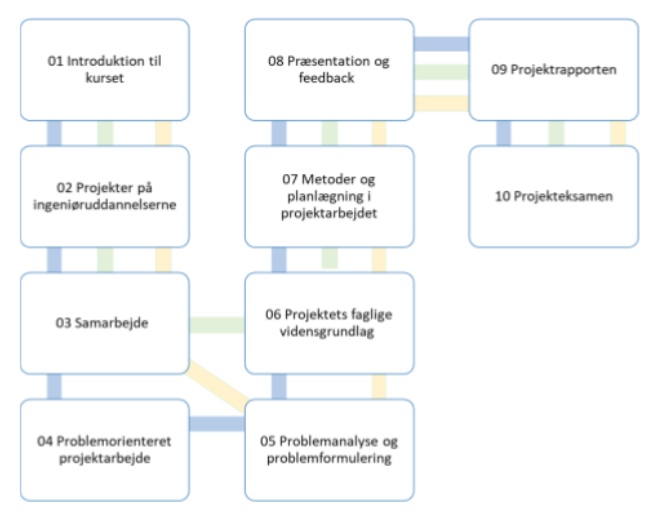
\includegraphics[width=12cm]{images/modulerne.png}
\caption{Modulerne i ProOnline}\label{fig:mod}
\end{center}
\end{figure}

%%%%%%%%%%%%%%%%%%%%%%%%%%%%%%%%%%%%%%%%%%%%%%%%%%%%%%%%%%%%%%%%%%%%%%%%%%%%%%%%
%%%%%%%%%%%%%%%%%%%%%%%%%%%%%%%%%%%%%%%%%%%%%%%%%%%%%%%%%%%%%%%%%%%%%%%%%%% Hvad indeholder et modul?

\section{Hvad indeholder et modul?}
Et modul introducerer dig til et emne og giver dig opgaver. Du får opgaver hvor du selv arbejder med stoffet, og opgaver hvor du tester eller overvejer din viden. Disse opgaver lægger op til en dialog med dine medstuderende og din projektvejleder, når I mødes i projektgruppen. Dialogen er et vigtigt element i online-kurset, fordi den giver dig en mulighed for at udvikle din viden og dine holdninger. Dialogen er også en bro over til selve projektarbejdet.

Hvert modul har en introduktion, individuelle opgaver, refleksionsopgave og et oplæg til dialog. Se figuren \ref{fig:indhold}:

\begin{figure}[h]
\begin{center}
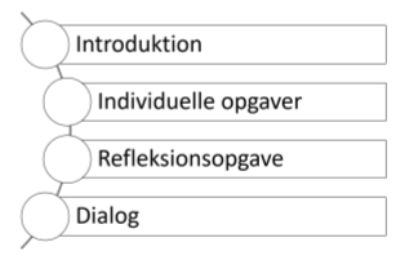
\includegraphics[width=10cm]{images/moduleindhold.png}
\caption{Module Indhold}\label{fig:indhold}
\end{center}
\end{figure}

\textbf{Introduktionen} beskriver og forklarer emnet. Introduktionen medtager det helt essentielle ved emnet, og giver dig ofte noget, som du ikke kan læse dig til i litteraturen.

\textbf{Individuelle opgaver} omfatter individuelt studie af litteratur eller andet, som uddyber den forklaring, der er givet i introduktionen, individuel træning vha. små illustrative træningsopgaver eller opgaver rettet mod et aktuelt projektforløb.

\textbf{Refleksionsopgaven} giver dig mulighed for at reflektere over det du har lært gennem igennem skrivning af et blogindlæg, muddiest points besvarelse af en RAT (Readiness Assurance Test) eller lignende.

\textbf{Dialog} giver dig et oplæg til en dialog med din projektgruppe og din vejleder, når I mødes. Du tager dine resultater af de individuelle opgaver og din refleksion med til drøftelse med din gruppe og din vejleder.

Din gennemførsel af et modul skal \textbf{godkendes}. Et modul bliver godkendt når du gennemfører opgaverne i det.

%%%%%%%%%%%%%%%%%%%%%%%%%%%%%%%%%%%%%%%%%%%%%%%%%%%%%%%%%%%%%%%%%%%%%%%%%%%%%%%%
%%%%%%%%%%%%%%%%%%%%%%%%%%%%%%%%%%%%%%%%%%%%%%%%%%%%%%%%%%%%%%%%%%%%%%%%%%% Hvad er “Muddiest Points”?

\section{Hvad er “Muddiest Points”?}
Muddiest Point handler om at få en hurtig indfangning af hvad der er svært eller forvirrende i forbindelse med en forelæsning eller studie. Her bruger vi det til, at studerende bruger et par minutter på at skrive, hvad der var det sværeste eller mest forvirrende ved modulet.

Fordelen ved Muddiest Points er, at det er nemt for de studerende at tage deres overvejelser med til drøftelse i projektgruppen og med projektvejlederen. For vejleder er det også nemt at skaffe sig et hurtigt overblik over, hvor skoen trykker.

%%%%%%%%%%%%%%%%%%%%%%%%%%%%%%%%%%%%%%%%%%%%%%%%%%%%%%%%%%%%%%%%%%%%%%%%%%%%%%%%
%%%%%%%%%%%%%%%%%%%%%%%%%%%%%%%%%%%%%%%%%%%%%%%%%%%%%%%%%%%%%%%%%%%%%%%%%%% Hvad er RAT (Readiness Assurance Test)?

\section{Hvad er RAT (Readiness Assurance Test)?}

\textbf{Readiness Assurance Test (RAT) er et værktøj i en Readiness Assurance Process (RAP)}.

\textbf{RAP} handler om at bliver klar til en læringsaktivitet. Vi bruger RAP til at sikre, at projektgruppe-medlemmerne forstår de grundlæggende begreber, definitioner og har den grundlæggende viden, som de har brug for mht projektarbejdet.

\textbf{RAP} har fem faser:

\textbf{Fase 1:} Individuelt studie af læsestof samt løsning af evt. opgaver

\textbf{Fase 2:} Individuel Readiness Assurance Test (iRAT) - (ca. 30 minutter): Test med multiple choice (evt. multiple svar) spørgsmål baseret på det læste materiale. Besvares uden at slå op i læsestoffet.

\textbf{Fase 3:} Team Readiness Assurance Test (tRAT) - (ca. 30 minutter): De samme spørgsmål drøftes og besvares i projektgrupperne.

\textbf{Fase 4:} Appelproces (evt) - (ca. 10 minutter): Teams opfordres til at appellere spørgsmålet, hvis de har et andet svar end vejlederens og har grund til at tro, at vejlederens svar er forkert.

\textbf{Fase 5:} Afklaring + diskussion - (Efter behov, f.eks. ca. 30 minutter): Efter behov afklarer og diskuterer vejleder/underviser stoffet sammen med de studerende.

I en \textbf{RAP} indgår der altså én multiple choice-test, som tages to gange: Første gang tages testen individuelt, og anden gang tages den samme test igen i projektgrupperne. Det er vigtigt, at gruppedelen ikke blot har karakter af en afstemning, men snarere har karakter af argumentation og diskussion. Det er simpelt, men har en stor virkning.

%%%%%%%%%%%%%%%%%%%%%%%%%%%%%%%%%%%%%%%%%%%%%%%%%%%%%%%%%%%%%%%%%%%%%%%%%%%%%%%%
%%%%%%%%%%%%%%%%%%%%%%%%%%%%%%%%%%%%%%%%%%%%%%%%%%%%%%%%%%%%%%%%%%%%%%%%%%% Hvordan får du fat i dine RAT-svar eller andre afleveringer?

\section{Hvordan får du fat i dine RAT-svar eller andre afleveringer?}
Du kan få fat i dine afleveringer ved at vælge Status og opfølgning i kursus-menuen. Det fører dig til en side, hvor du kan se mere om dine afleveringer.

%%%%%%%%%%%%%%%%%%%%%%%%%%%%%%%%%%%%%%%%%%%%%%%%%%%%%%%%%%%%%%%%%%%%%%%%%%%%%%%%
%%%%%%%%%%%%%%%%%%%%%%%%%%%%%%%%%%%%%%%%%%%%%%%%%%%%%%%%%%%%%%%%%%%%%%%%%%% Hvordan kommer du i gang og hvordan arbejder du med kurset?

\section{Hvordan kommer du i gang og hvordan arbejder du med kurset?}
Du gennemfører kurset ved at gennemfører kursets moduler. Hvert modul er lavet som en læringssti, og de enkelte elementer åbner derfor efterhånden, som du arbejder dig igennem modulet. Det vil tage dig mellem ½ time og 4 timer at gennemføre et modul.

Du starter ved at klikke på \textbf{Planer} og dernæst klikke på det første modul. Du kan arbejde dig igennem kurset i dit eget tempo, blot du overholder de tidsfrister, der er sat op af din uddannelse, og som er bestemt af semesterprojektets forløb.

Du kan altid vende tilbage til et modul. Du går blot igen ind under Planer og klikker på det modul, som du ønsker at genoptage. Du kan også genfinde oplysninger fra et modul under \textbf{Ressourcer}.

\end{document}
